\documentclass[notes,slidesec,a4]{seminar}

\usepackage[utf8]{inputenc}
\usepackage[spanish]{babel} % espanol


\usepackage{t-gsyc-6}
\usepackage{fancybox}
\usepackage{graphics}
\usepackage{moreverb}
\usepackage{alltt}
\usepackage{html}
\usepackage{color}
\usepackage[usenames,dvipsnames,svgnames,table]{xcolor}
\usepackage{amsmath}
\usepackage[normalsize]{subfigure}
\usepackage{url}
\usepackage{hyperref}
\usepackage{listings}
\usepackage{multirow}


\title{MANEJO DE UN DRONE CON
%\\ \vspace{0.2cm} 
 WEBRTC Y JDEROBOT}
\author{Iván Rodríguez-Bobada Martín}

\cop{Iván Rodríguez-Bobada Martín}
\address{i.rodriguezmar@alumnos.urjc.es}

\begin{document}
\maketitle

%%--------------------------------------------------------------

\begin{hslide}
\slsect{Índice}
\begin{itemize}
\item Introducción 
\item Objetivos
\item Infraestructura software
\item Desarrollo software
\item Experimentos
\item Conclusiones
\end{itemize}
\end{hslide}


%%--------------------------------------------------------------

\begin{hslide}
\slsect{Introducción}
\slsubsect{Aplicaciones de los drones}
\begin{minipage}[t]{0.5\textwidth}
\begin{center}
\begin{figure}
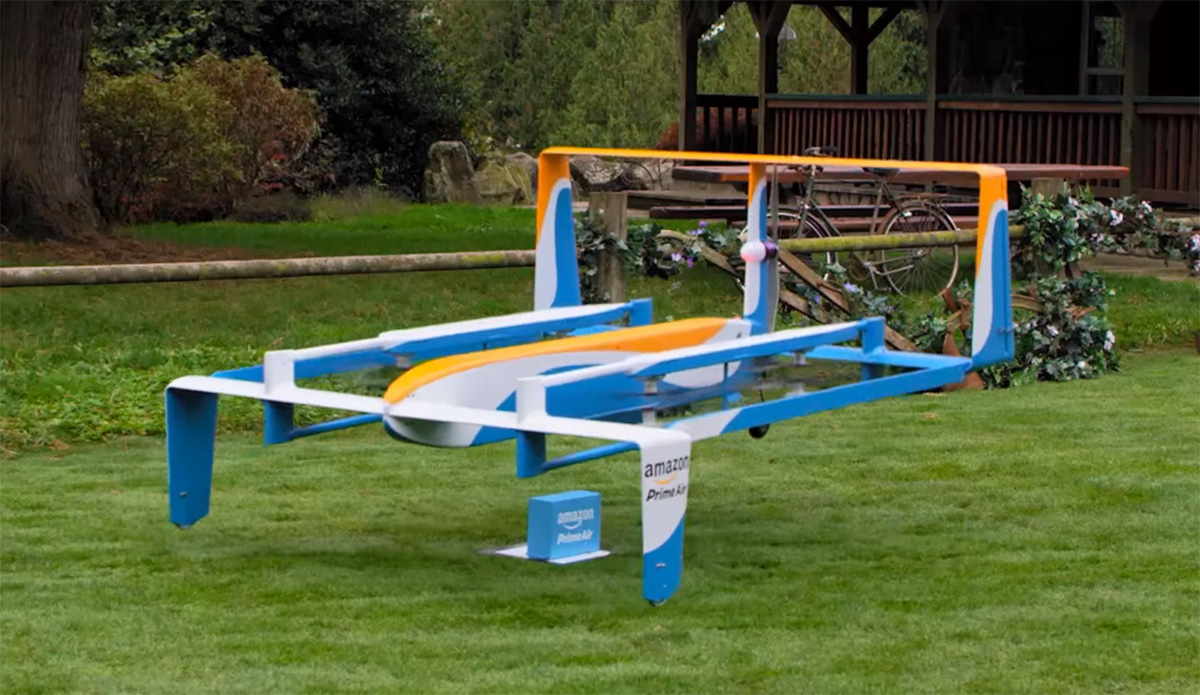
\includegraphics[width=0.6\textwidth]{img/amazon}
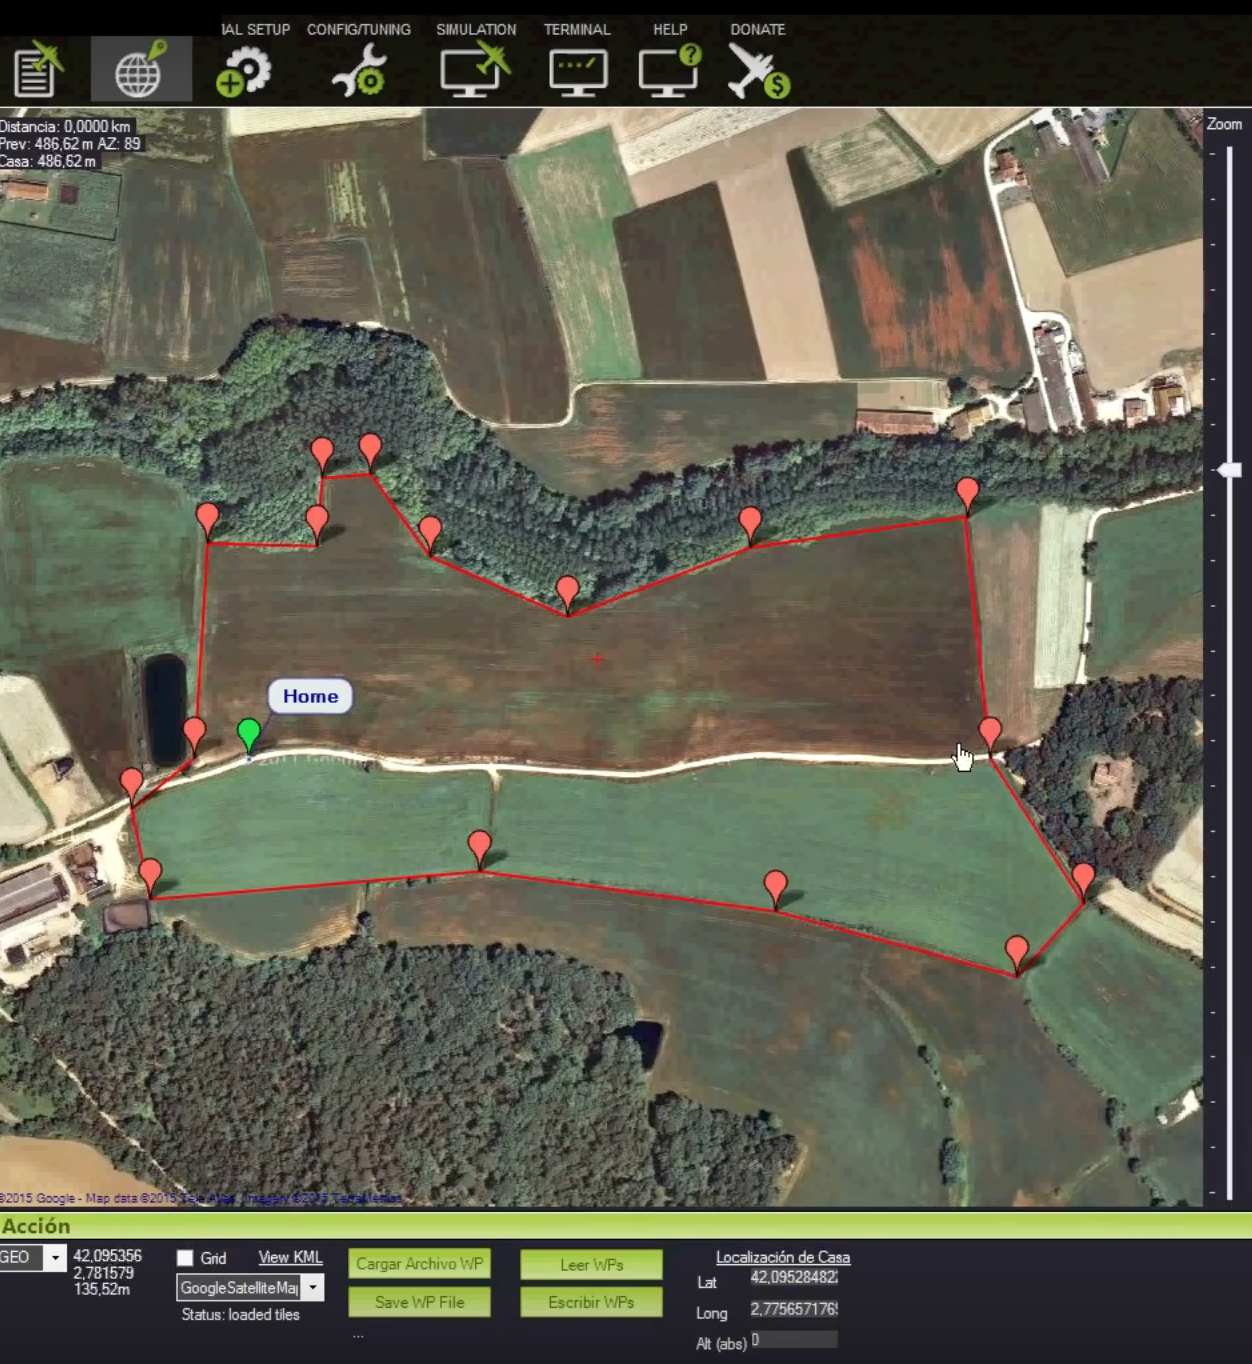
\includegraphics[width=0.6\textwidth]{img/hemav1}
\end{figure}
\end{center}
\end{minipage}
\begin{minipage}[t]{0.5\textwidth}
\begin{center}
\begin{figure}
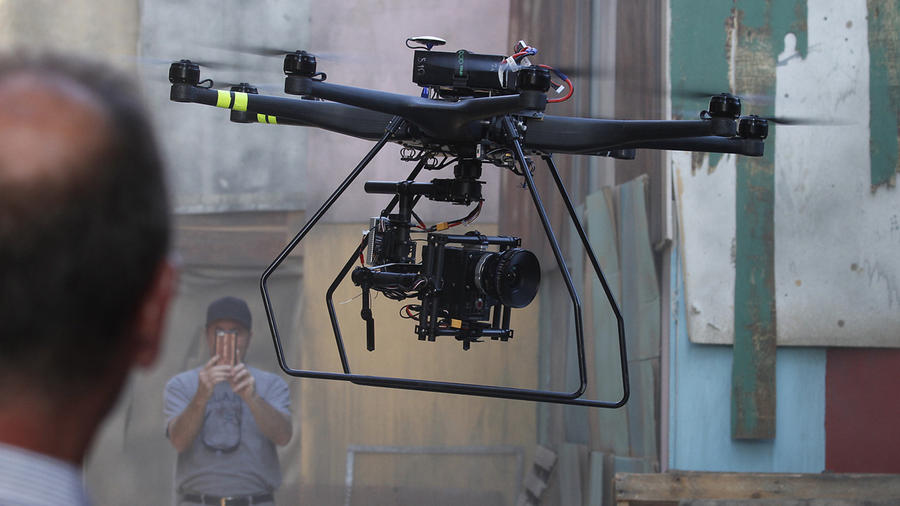
\includegraphics[width=0.8\textwidth]{img/dronefilm}
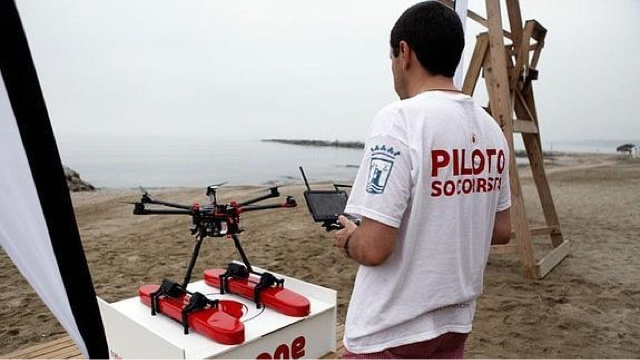
\includegraphics[width=0.8\textwidth]{img/socorrista}
\end{figure}
\end{center}
\end{minipage}
\end{hslide}

%%--------------------------------------------------------------


\begin{hslide}
\slsubsect{Antecedentes: Surveillance 5.1}
\begin{itemize}
\item Es el TFG de Edgar Barrero.
\item Está desarrollado con Ruby on Rails.
\item Un servidor web intermedio se conecta a los servidores ICE.
\end{itemize}
\begin{minipage}[t]{0.3\textwidth}
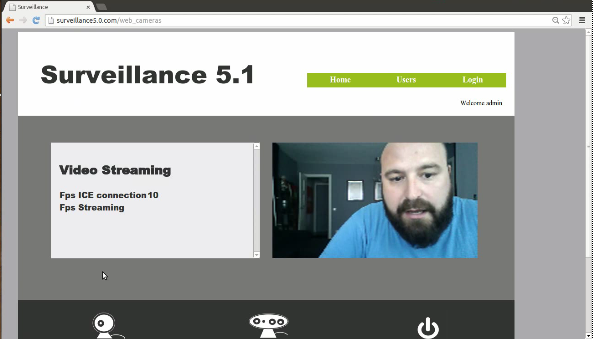
\includegraphics[width=\textwidth]{img/surveillance5}
\end{minipage}
\begin{minipage}[t]{0.7\textwidth}
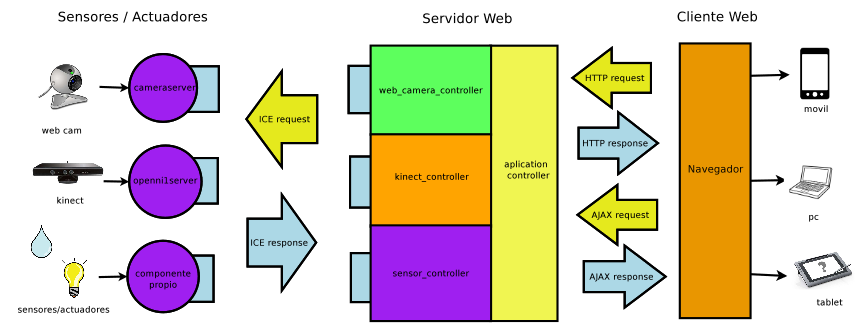
\includegraphics[width=\textwidth]{img/esquema_s5}
\end{minipage}
\end{hslide}


%%--------------------------------------------------------------


\begin{hslide}
\slsubsect{Antecedentes: Teleoperadores y visores Web en JdeRobot}
\begin{itemize}
\item Es el TFG de Aitor Martínez.
\item Está desarrollado directamente en el navegador con JavaScript.
\item Conexión con sensores y actuadores sin servidores intermedios.
\end{itemize}
\begin{center}
\begin{figure}
\includegraphics[width=0.7\textwidth]{img/uavviewerjs_aitor}
\end{figure}
\end{center}
\end{hslide}

%%--------------------------------------------------------------

\begin{hslide}
\slsect{Objetivo}
Teleoperar un drone con tecnologías web de última generación
sin servidores intermedios desde multidispositivos.

Sub-objetivos:
\begin{itemize}
\item Conexión local: par local - drone.
\item Conexión remota entre pares: par local - par remoto.
\item Interfaz web de usuario amigable e intuitiva.
\end{itemize}
\end{hslide}

%%--------------------------------------------------------------

\begin{hslide}
\slsect{Infraestructura software}
\slsubsect{ArDrone de Parrot}
\begin{itemize}
\item Drone sobre el que se basa el proyecto.
\item Se ha usado la versión ArDrone 2.0. 
\end{itemize}

\begin{center}
\begin{figure}
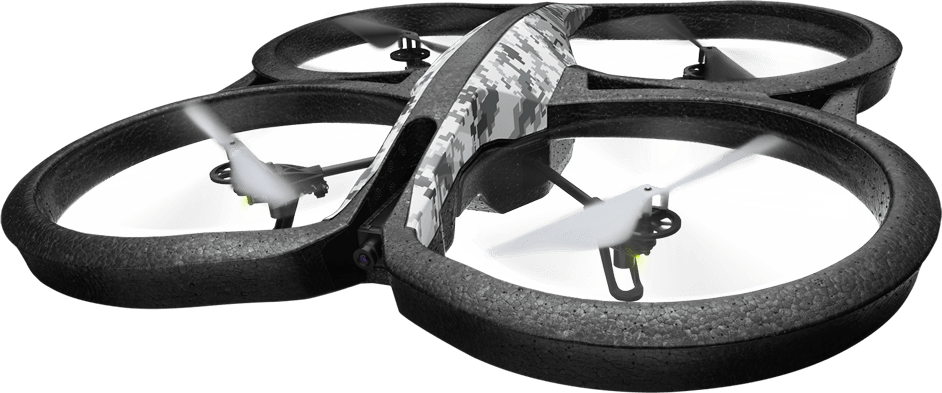
\includegraphics[width=0.6\textwidth]{img/ardrone}
\end{figure}
\end{center}
\end{hslide}

%%--------------------------------------------------------------

\begin{hslide}
\slsubsect{Gazebo e ICE}
\begin{itemize}
\item \textbf{Gazebo}: Simula sensores, actuadores, etc del ArDrone en un mundo virtual.
\item \textbf{ICE}: Permite comunicaciones \textit{cross-language} y \textit{cross-platform}.
\end{itemize}

\begin{center}
\begin{figure}
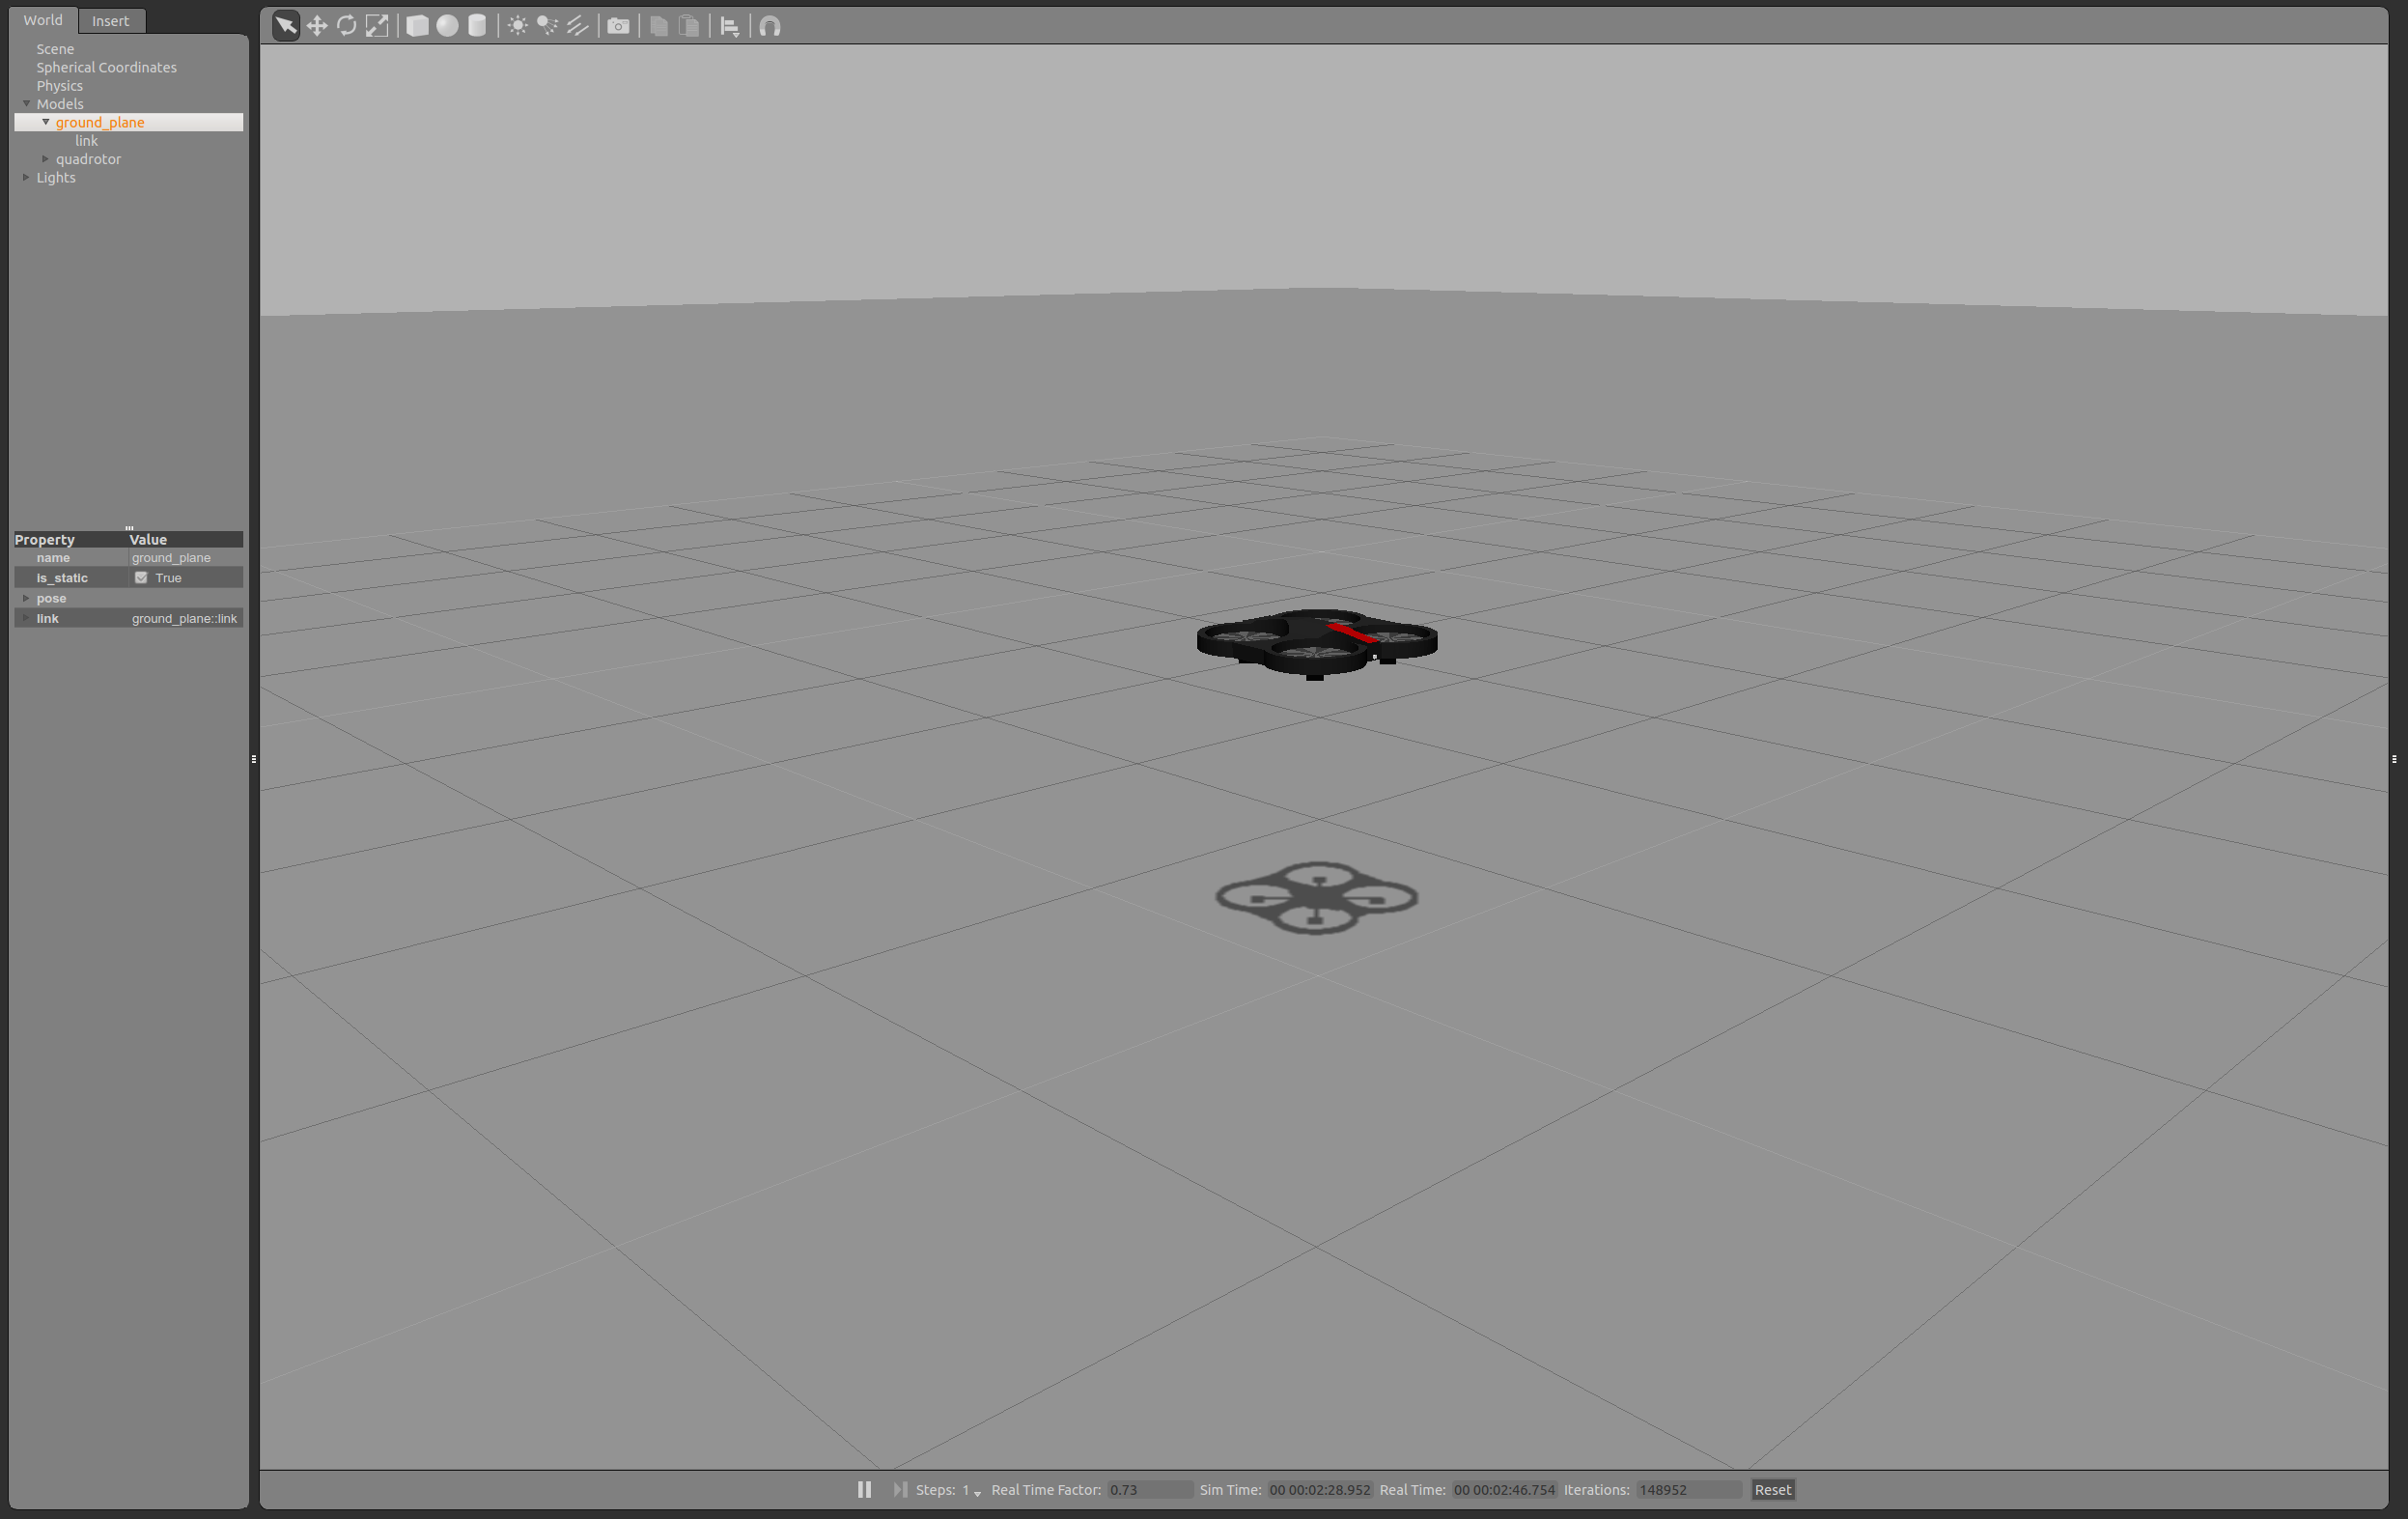
\includegraphics[width=0.6\textwidth]{img/gazebo}
\end{figure}
\end{center}
\end{hslide}


%%--------------------------------------------------------------

\begin{hslide}
\slsubsect{JdeRobot}
\begin{minipage}[t]{0.7\textwidth}
\begin{itemize}
\item Simplifica el acceso a unidades hardware.
\item Se han usado dos herramientas:
\begin{itemize}
\item \emph{Plugin de Gazebo}: Versión virtual del drone ArDrone de Parrot.
\item \emph{ArDroneServer}: Servidor que se comunica directamente con el drone.
\end{itemize}
\end{itemize}

\end{minipage}
\begin{minipage}[t]{0.3\textwidth}
\begin{center}
\begin{figure}

\includegraphics[width=0.8\textwidth]{img/jderobot}
\end{figure}
\end{center}
\end{minipage}
\end{hslide}

%%--------------------------------------------------------------


\begin{hslide}
\slsubsect{WebRTC}
\begin{itemize}
\item Tecnología web que permite comunicaciones entre navegadores en tiempo real.
\item Transmisión de audio, vídeo y datos.
\item Sin necesidad de servidores intermedios.
\end{itemize}
\end{hslide}

%%--------------------------------------------------------------


\begin{hslide}
\slsect{Desarrollo software}
\begin{center}
\begin{figure}
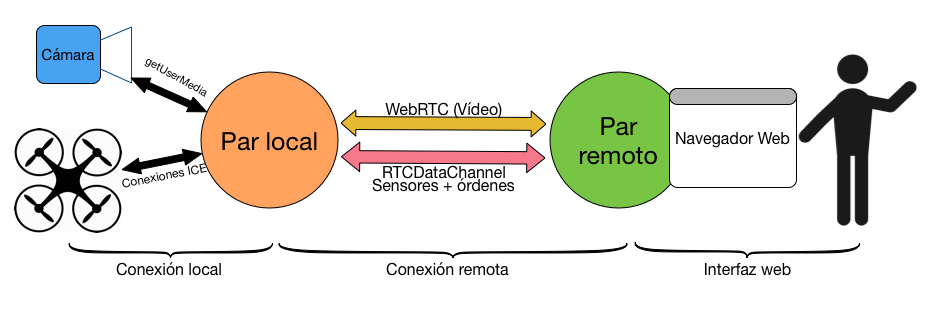
\includegraphics[width=1.1\textwidth]{img/esquema_general}
\end{figure}
\end{center}
\end{hslide}



%%--------------------------------------------------------------

\begin{hslide}
\slsubsect{Flujo de llamada del proyecto}
\begin{center}
\begin{figure}
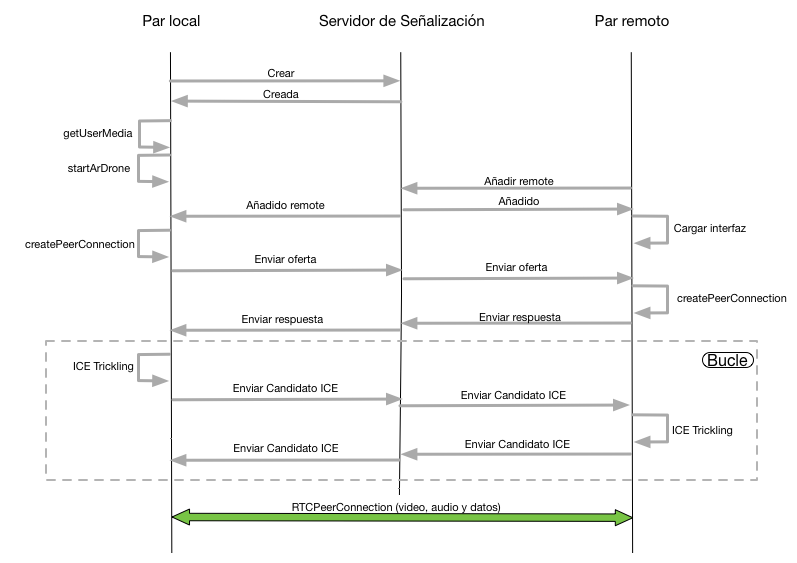
\includegraphics[width=0.8\textwidth]{img/diagrama_general}
\end{figure}
\end{center}
\end{hslide}

%%--------------------------------------------------------------

\begin{hslide}
\slsubsect{Conexión local}
\begin{itemize}
\item Esta conexión se divide en dos a su vez:
\begin{itemize}
\item \textbf{ArDroneServer y WebSockets:} Conexión que se establece entre el navegador y el drone.
\item \textbf{getUserMedia:} El navegador accede a la cámara utilizando la API de WebRTC.
\end{itemize}
\end{itemize}
\end{hslide}

%%--------------------------------------------------------------

\begin{hslide}
\slsubsect{Conexión local: ArDroneServer y WebSockets}
\begin{itemize}
\item Para establecer la conexión hay que activar los WebSockets de ICEJS en el archivo de configuración del servidor ArDroneServer.
\end{itemize}
\lstset{}
\begin{lstlisting}
 Ice.Plugin.IceWS=IceWS:createIceWS
\end{lstlisting}
\end{hslide}

%%--------------------------------------------------------------


%%--------------------------------------------------------------


%%--------------------------------------------------------------


%%--------------------------------------------------------------



\end{document}